\iffalse
\section*{Preface}

The sun has set over the Olympics on what is undoubtedly one of the last clear days of the year.
Seattle is beautiful in the summer, but I've always preferred the rain -- the persistent grey sidesteps the feeling of dissonance that accompanies sunny weather.
It is only fitting, then, that this document, which is the culmination of my time here, will be written over the long nights of a Pacific northwest winter.  

\vspace{.5em}
October 30, 2021
\vspace{-.7em}

Chinatown/International District
\vspace{-.7em}

Seattle, Washington

\begin{verse}
\textbf{Promise}

Long nights, short years. Forgiving
\\
silence.

When morning comes, and pain --

no one is a stranger, this whole world is your home. 
\end{verse}
\fi

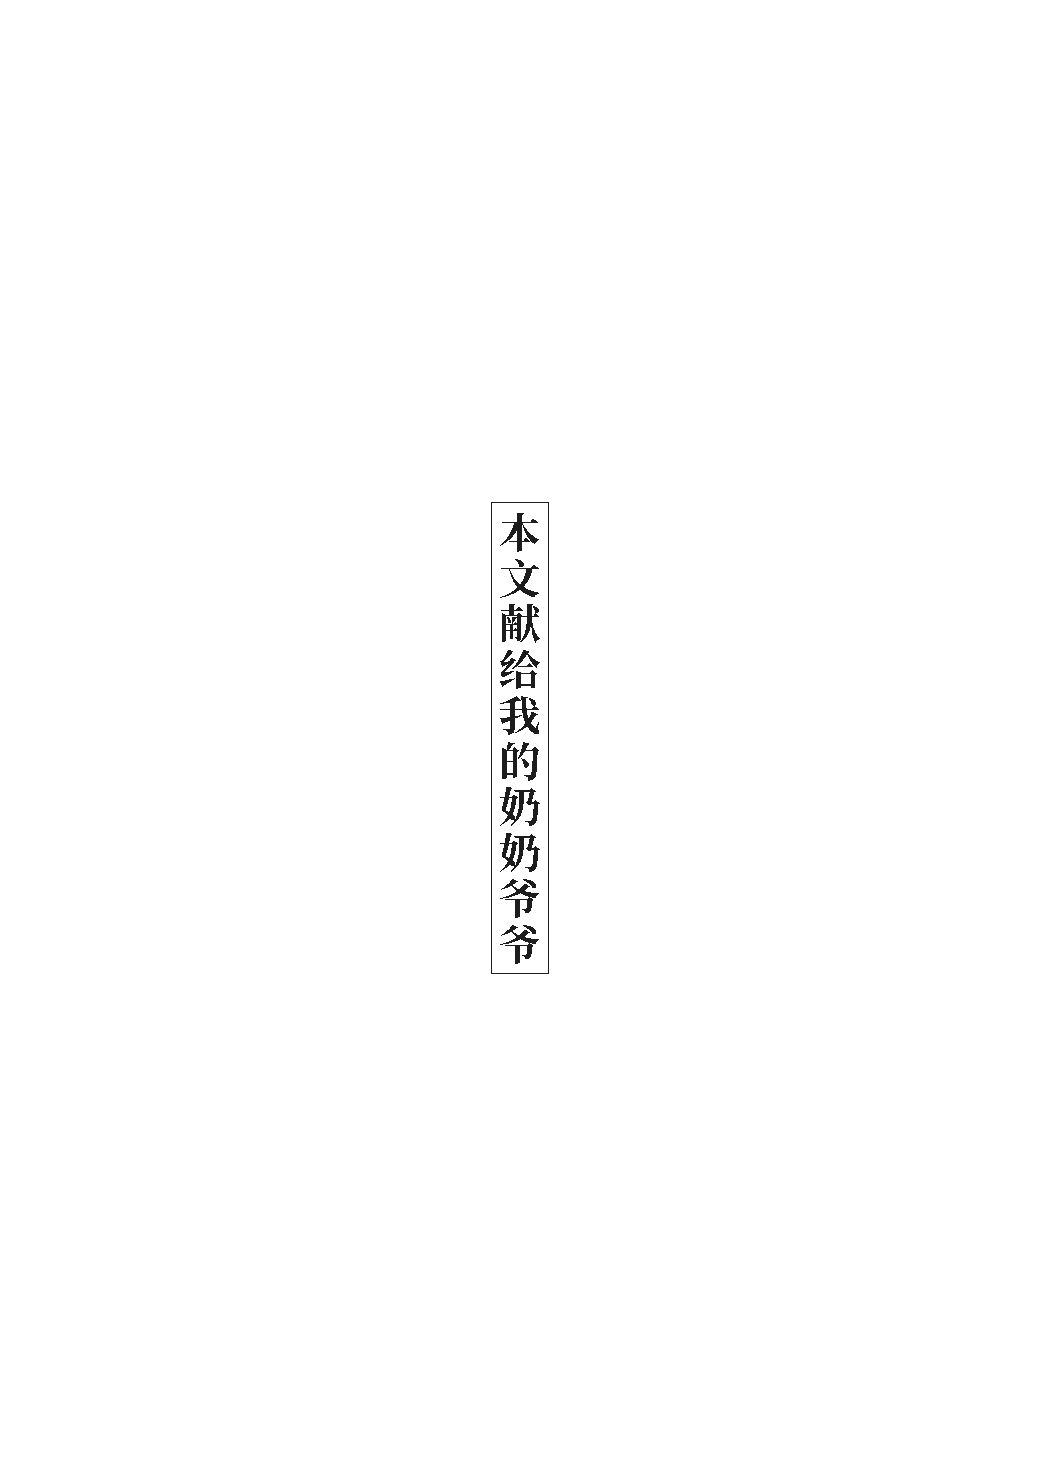
\includepdf[]{special_pages/dedication_plain.pdf}

\section*{Preface}

At night, my apartment looks out to a thousand illuminated windows.
I'm drawn such views because they make me feel an isolating sense of closeness; behind each window is a person---a family enjoying dinner, a student working on their homework, a cleaning person ending their shift.
I do not know them and they do not know me, yet we are all connected in this moment of existence. 
This is \emph{sonder}, a concept for which we find a definition in the Dictionary of Obscure Sorrows:
\begin{quote}
\textbf{sonder}

{\textit n.} the realization that each random passerby is living a life as vivid and complex as your own%---populated with their own ambitions, friends, routines, worries and inherited craziness---an epic story that continues invisibly around you like an anthill sprawling deep underground, with elaborate passageways to thousands of other lives that you’ll never know existed, in which you might appear only once, as an extra sipping coffee in the background, as a blur of traffic passing on the highway, as a lighted window at dusk.
\end{quote}

Sonder, even with the accompanying melancholy, has been the single most consistent force driving my success throughout my tertiary education.
It only fitting, then, that it receives mention in my dissertation, the symbolic culmination of my formal education.


%In a sense, this thesis is the culmination of my formal education.

%Surprisingly minimal requirements regarding the formatting of 

\iffalse
I continually find myself chasing certain aesthetic emotions.
After hours, sonder is perhaps the 


emotional aesthetic,

I hope this thesis invokes such 

editorial control.

This is expressed in two main ways. First, exposition

Second typesetting

but also in the typesetting and 
\fi

\begin{flushright}
\vspace{5em}
Chinatown/International District
\vspace{-.7em}

Seattle, Washington %2022
\end{flushright}




\clearpage
\section*{Acknowledgements}


First and foremost, I would like to thank my thesis advisors, Anne Greenbaum and Thomas Trogdon, whose support and guidance throughout my PhD have shaped me into the researcher I am today.
Many PhD students struggle to find a good advisor, but I had two excellent ones.
Anne, thank you for sharing with me your vast wisdom on numerical linear algebra and for always making time for me when I stopped by your office unannounced.
Tom, thank you for pushing me to produce work of the highest quality and for answering my many, perhaps repetitive, career advice questions.
I feel truly fortunate to have crossed path's with each of you, and I look forward to ongoing collaboration in the future.

Many others have contributed directly to my academic development.
I'm particularly grateful to my undergraduate advisor, Roger Tobin, for his mentorship throughout my time at Tufts.
This was a formative time in my life during which much of my current perspective on academia was developed.
%as well as to Megan Callow and everyone in the IWP. 
%Alexandra Elbakyan
I'm also thankful for the collaborators I've had over the past several years, Raghu Bollapragada, Erin Carson, Yu-Chen Cheng, Eric Hallman, Hexuan Liu, Cameron Musco, Christopher Musco, Shashanka Ubaru, Rachel Ward, Natalie Wellen, and Qichen Xu, each of who contributed, in one way or another, to the content of this thesis.
I especially want to thank Yu-Chen for teaching me much of what I know about probability during the first year of my PhD.
Finally, thanks to my thesis committee, Sasha Aravkin and Maryam Fazel, for contributing their time and energy to my thesis and defense.

I'm indebted to many folks at UW who supported me throughout my time here.
This includes everyone at Hall Health, upstairs and downstairs, the staff and faculty in the Applied Math department, and the many students who I regularly interacted with.
When I first vested the department as a prospective student, it was immediately clear that there was a wonderful community of students. 
This was the deciding factor in my decision to come to UW, and I have been continually grateful for this community throughout my time in the program. 
%I'd especially like to thank Andreas, Brian, and Jeremy for modeling what PhD student life could look like and for helping to foster the amath community during my first few years in the program.
I was also extremely blessed to have a wonderful cohort without whom the last five years would have been far less enjoyable.
%Thanks especially to Diya, Jorge, Katherine, Micah, Nora, Roman, and Ying-Jen for the many memories we made.


Finally, I want to acknowledge my family and friends.
This thesis is dedicated to my grandparents, 陈祖浩 and 鲁月娥, the greatest supporters of my education.
To my parents, Ming-Guang (陈明光) and Peggy, thank you for providing for me since before I was even born.
This achievement is as much yours as it is mine.
To my partner, 黃羿綺, I'm so happy our lives intersected when they did.
Thank you for the constant love and support, and for quarantining with me during the pandemic. 
I cannot imagine what the last few years would have looked like without you.
Last, a shout out to  Jesse, Matthew, Max, Tailong, and Vaibhav, my ``internet friends'', who have each been with me through many stages of my life, despite large geographic distances.

\vfill

This material is based on work supported by the National Science Foundation under grant number DGE-1762114.
Any opinion, findings, and conclusions or recommendations expressed in this material are those of the author and do not necessarily reflect the views of the National Science Foundation.

